
\begin{comment}
\begin{frame}{Proposal}

\begin{enumerate}
    \item Data Model
    \vspace{1em}
    \item Definition of Anomalous Patterns of Transactions
    \vspace{1em}
    \item Query Model
    \vspace{1em}
    \item Continuous Query Engine - $\mathsf{DP_{ATM}}$
    \vspace{1em}
    \item Architecture
\end{enumerate}
\end{frame}
\end{comment}

\begin{frame}{Proposal: Data Model}
    \centering
    \hspace*{-0.5cm}
    \begin{tikzpicture}
        \node  (0) at (0, 0) {\textbf{\emph{Continuously Evolving Database}}};
        \node [below left=0.5cm and 0.1cm of 0] (1) {\textcolor{blue}{Stable}};
        \node [below right=0.5cm and 0.1cm of 0] (2) {\textcolor{blue}{Volatile}};
        \node [below=1cm of 1] (3) {Central Bank Database};
        \node [below=1cm of 2] (4) {ATM Transactions Stream};
        \node [below=1cm of 3] (5) {Property Graph (PG)};
        \node [below=1cm of 4] (6) {Property Graph (PG)};
        \node [below=0.5cm of 5] (7) {Neo4j};
        \node [below=0.5cm of 6] (8) {Induced card subgraphs};
        \node [below=0.1cm of 7] (9) {\textit{(External)}};
        \node [below=0.1cm of 8] (10) {\textit{(Internal)}};
        \draw[style={tree_edge}]{} (0) to (1);
        \draw[style={tree_edge}]{} (0) to (2);
        \draw[style={tree_edge}]{} (1) to (3);
        \draw[style={tree_edge}]{} (2) to (4);
        \draw[style={tree_edge}]{} (4) to (6);
        \draw[style={tree_edge}]{} (3) to (5);
        \draw[style={tree_edge}]{} (6) to (8);
        \draw[style={tree_edge}]{} (5) to (7);
    \end{tikzpicture}

\end{frame}

\begin{comment}
\begin{frame}{Proposal: Data Model}

\begin{itemize}
\item Nature of our data: ATM transactions on a bank system.
%\item[$\Rightarrow$] \textcolor{red}{Dynamic} data sources. Transactions occur continuously.
\vspace{2em}
\pause
\item \textbf{\emph{Continuously evolving database}} - data can be stable and volatile.
\begin{itemize}
    \vspace{0.5em}
    \item[$\Rightarrow$] Graph Data Model: Property Graph (PG).
    \vspace{1em}
    \item[$\Rightarrow$] Graph Database System: Neo4j (based on PG).
\end{itemize}
\end{itemize}
\end{frame}
\end{comment}

\begin{frame}{Proposal: Data Model}
    \begin{columns}
        % First Column (Stable PG)
        \column{0.5\textwidth}
        \begin{center}
            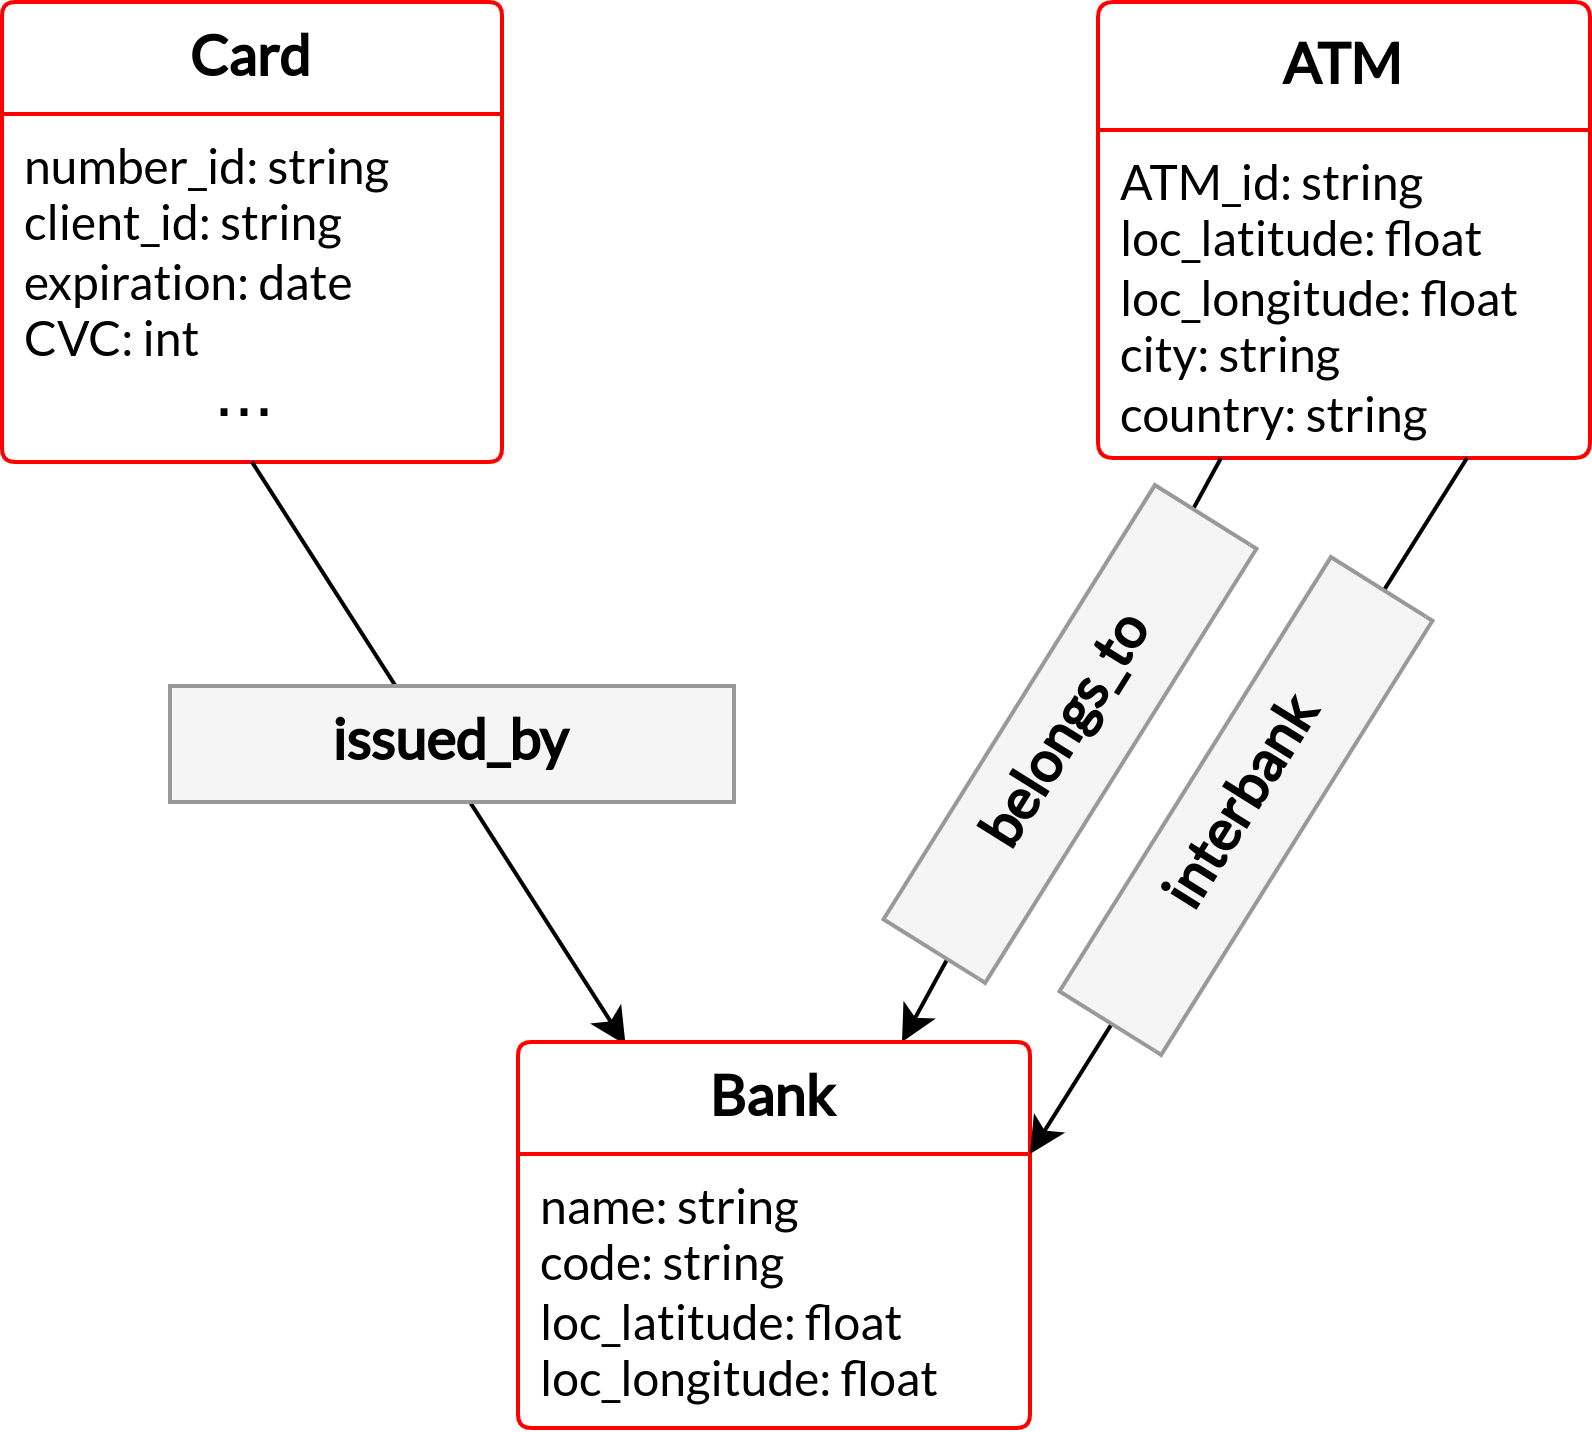
\includegraphics[width=1.0\textwidth]{figures/stable-presentacion-1.png}  
        \end{center}

        % Second Column (Volatile PG)
        \column{0.5\textwidth}
        \begin{center} 
            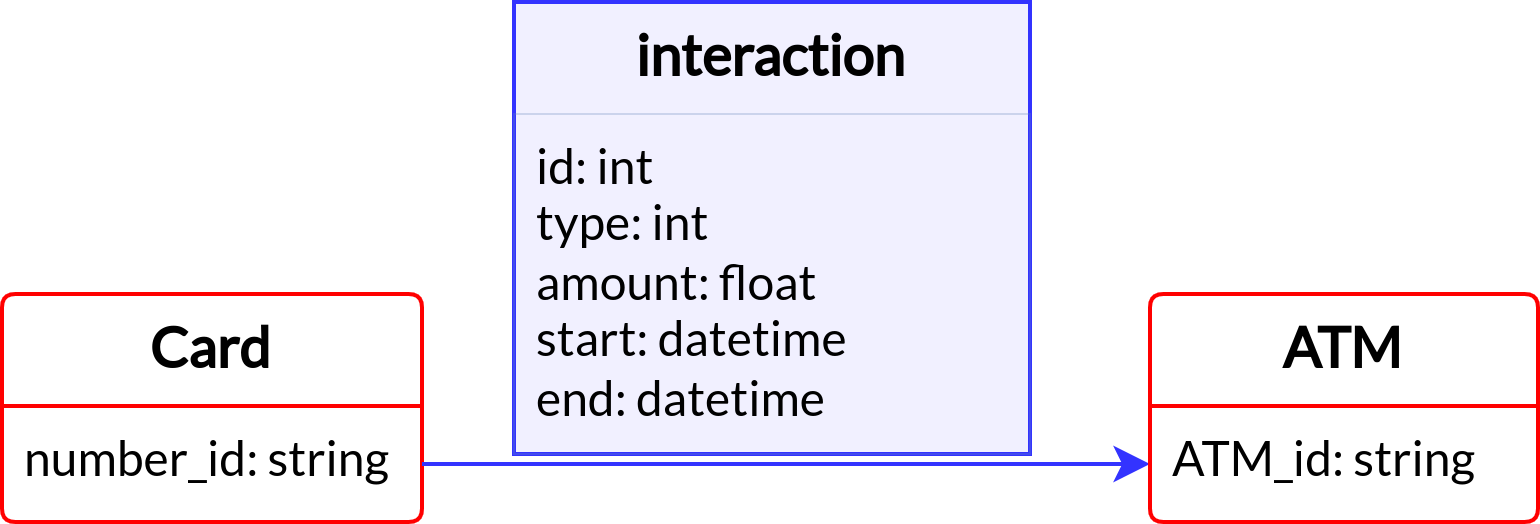
\includegraphics[width=1.0\textwidth]{figures/volatile-presentacion-1.png}
        \end{center}
    \end{columns}
    \vspace{0.6em}
    \begin{columns}
        \column{0.5\textwidth}
        \hspace{4.7em}\textcolor{blue}{Stable PG} \\Central bank database 
        {\small(\emph{persistent relations of standard graph dbs).}}
        \column{0.5\textwidth}
        \hspace{4.7em}
        \textcolor{blue}{Volatile PG} \\
        \vspace{0.3em}
        Transactions 
        {\small(\emph{non-persistent relations. Edges in the data stream).
        \textbf{Induce subgraphs used to perform query evaluation}}}
    \end{columns}
    
\end{frame}


\begin{comment}
\begin{frame}{Proposal: Data Model}

\only<1>{
\begin{itemize}
    \item [$\Rightarrow$] Stable PG
    \begin{itemize}
    \item Models the data a bank typically gathers on cards, ATMs...
    \end{itemize}
\end{itemize}
}

\only<2>{
\begin{itemize}
    \item [$\Rightarrow$] Volatile PG
    \vspace{0.2em}
    \begin{itemize}
        \item Volatile relations (transactions) are the \textcolor{red}{edges arriving in data streams} during a set time interval. 
        \item \textcolor{red}{Induce subgraphs} that exist only while the relations are still valid.
    \end{itemize}
\end{itemize}
}

\begin{figure}
    \centering
    \only<1>{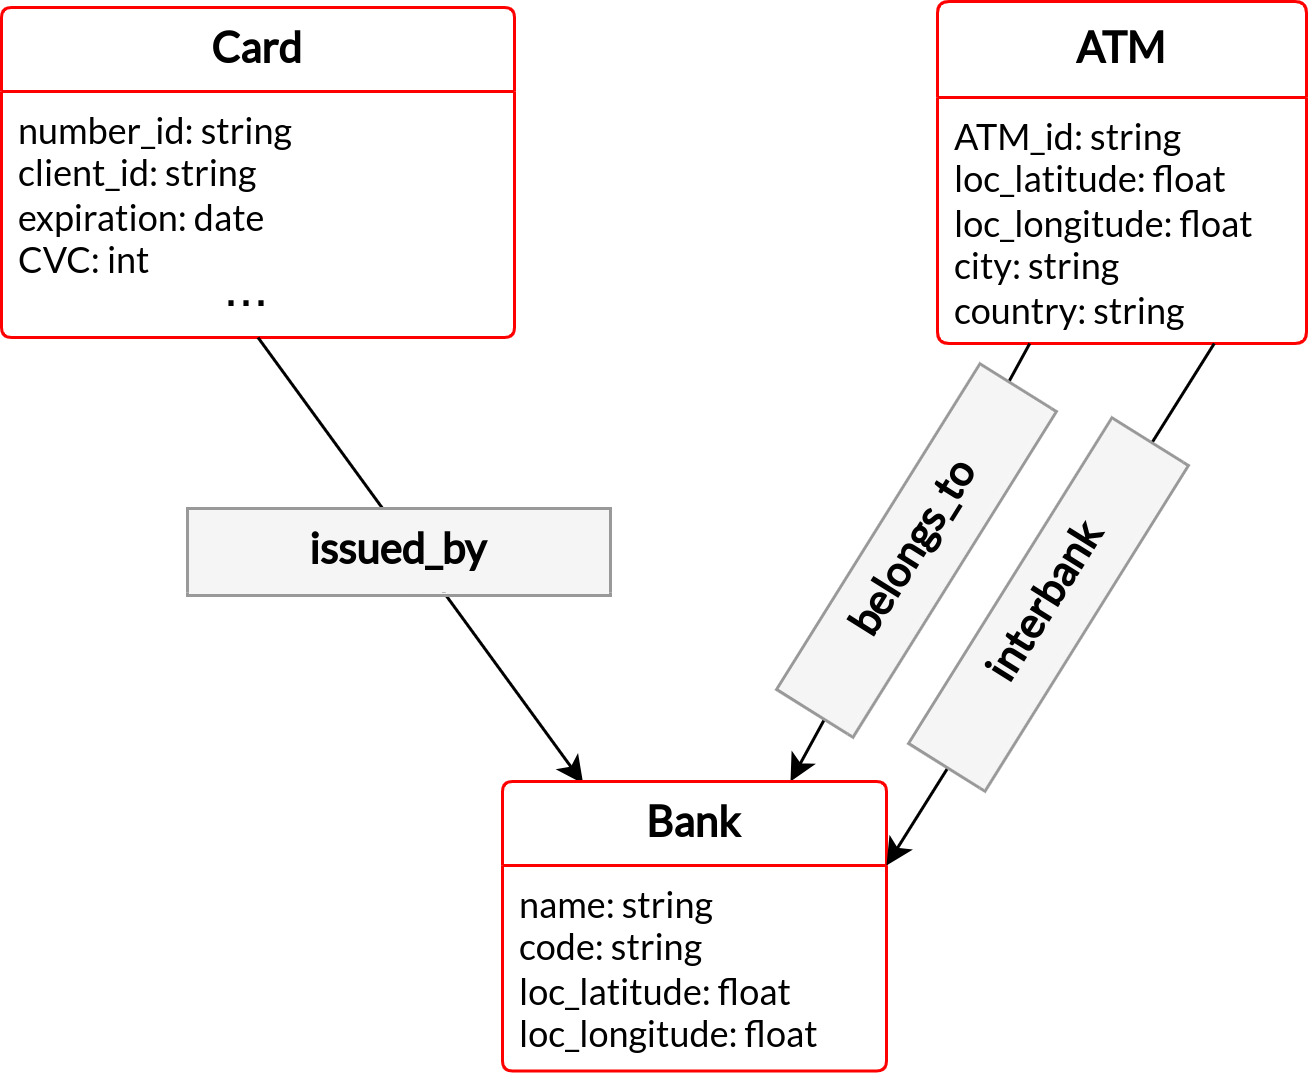
\includegraphics[width=0.65\textwidth]{figures/stable-presentacion.png}}
    \only<2>{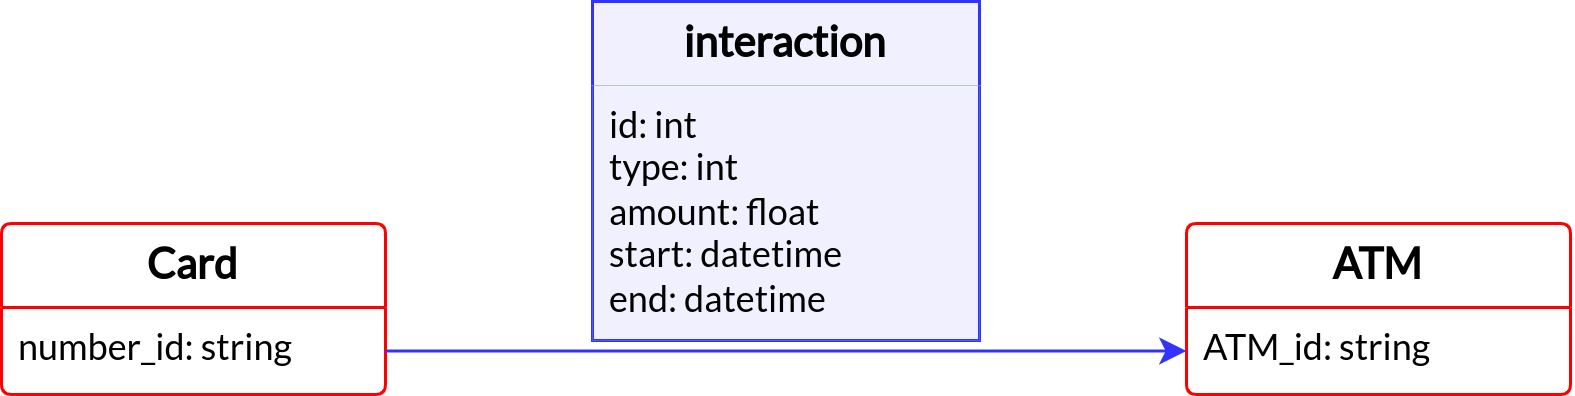
\includegraphics[width=0.8\textwidth]{images/1-DataModel/schema-volatile.png}}
\end{figure}

\end{frame}
\end{comment}


\begin{comment}
\begin{frame}{The data model: Stable PG}

\begin{figure}
    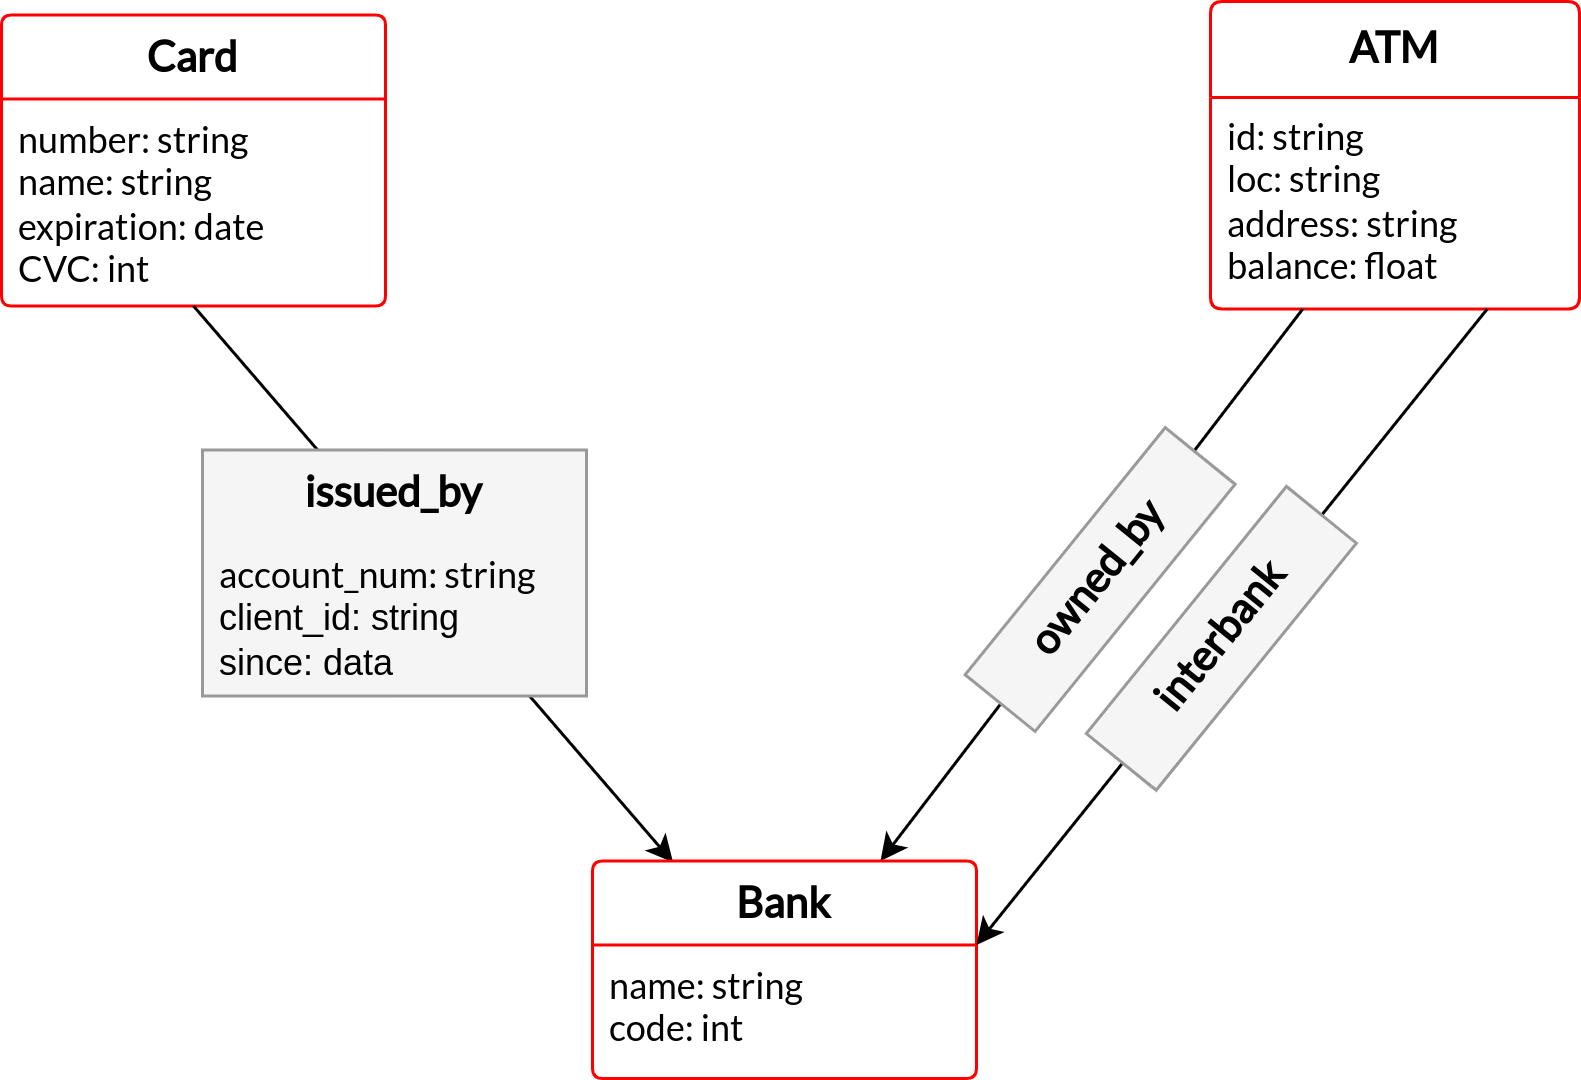
\includegraphics[width=0.8\textwidth]{figures/stable.png}
\end{figure}

\begin{itemize}
    \item Models the data a bank typically gathers on cards, ATMs...
\end{itemize}
\end{frame}

\begin{frame}{The data model}
\begin{figure}
    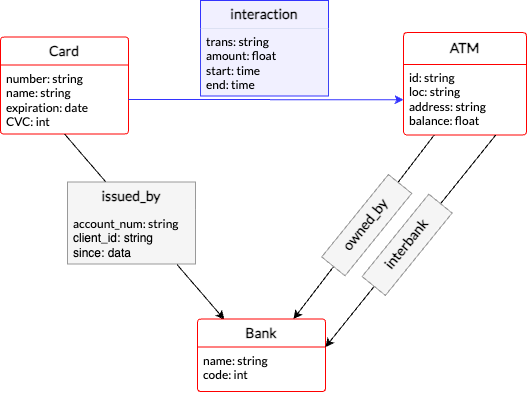
\includegraphics[width=0.9\textwidth]{figures/schema.png}
\end{figure}
\end{frame}

\begin{frame}{The data model: Volatile PG}

\begin{figure}
    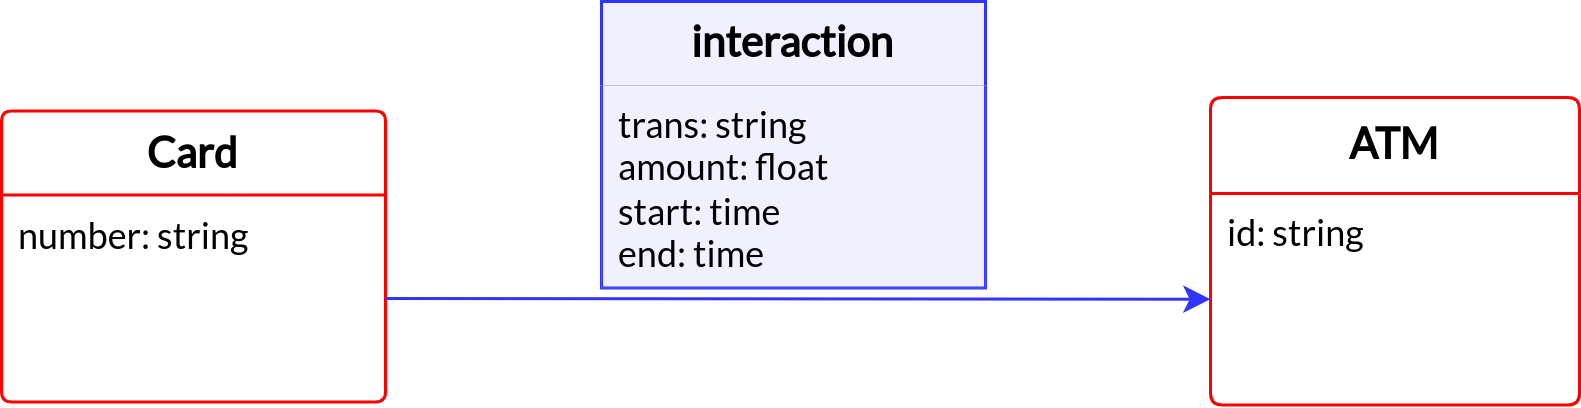
\includegraphics[width=0.9\textwidth]{figures/volatile.png}
\end{figure}

\begin{itemize}
    \item Models the interactions between cards and ATM entities.
    \item Volatile relations (transactions) are the edges arriving in data streams during a set time interval. 
    \item Induce subgraphs that exist only while the relations are still valid.
    \item Minimal information (only identifiers) on its nodes. 
\end{itemize}

\end{frame}

\begin{frame}{The data model: Volatile subgraph}
\textbf{Note}: Creation of 2 edges per transaction - the \emph{opening} edge and the \emph{closing} edge.
\textbf{Important} for some anomalous query patterns, to detect them before they are completely committed. 

\begin{figure}
    \centering
    \only<1>{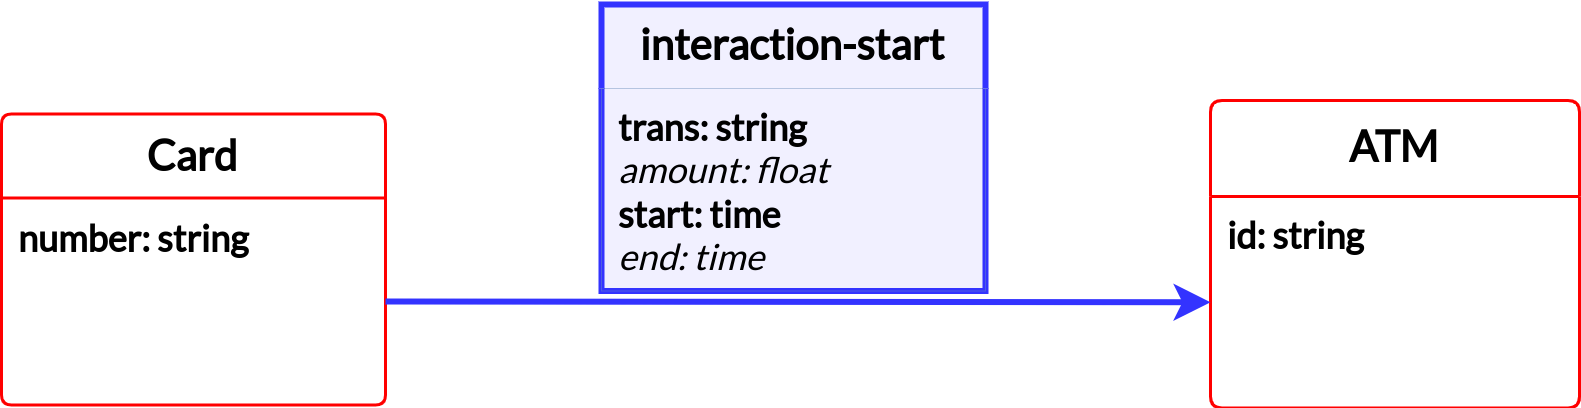
\includegraphics[width=\textwidth]{figures/2-edges-tx-start.png}}
    \only<2>{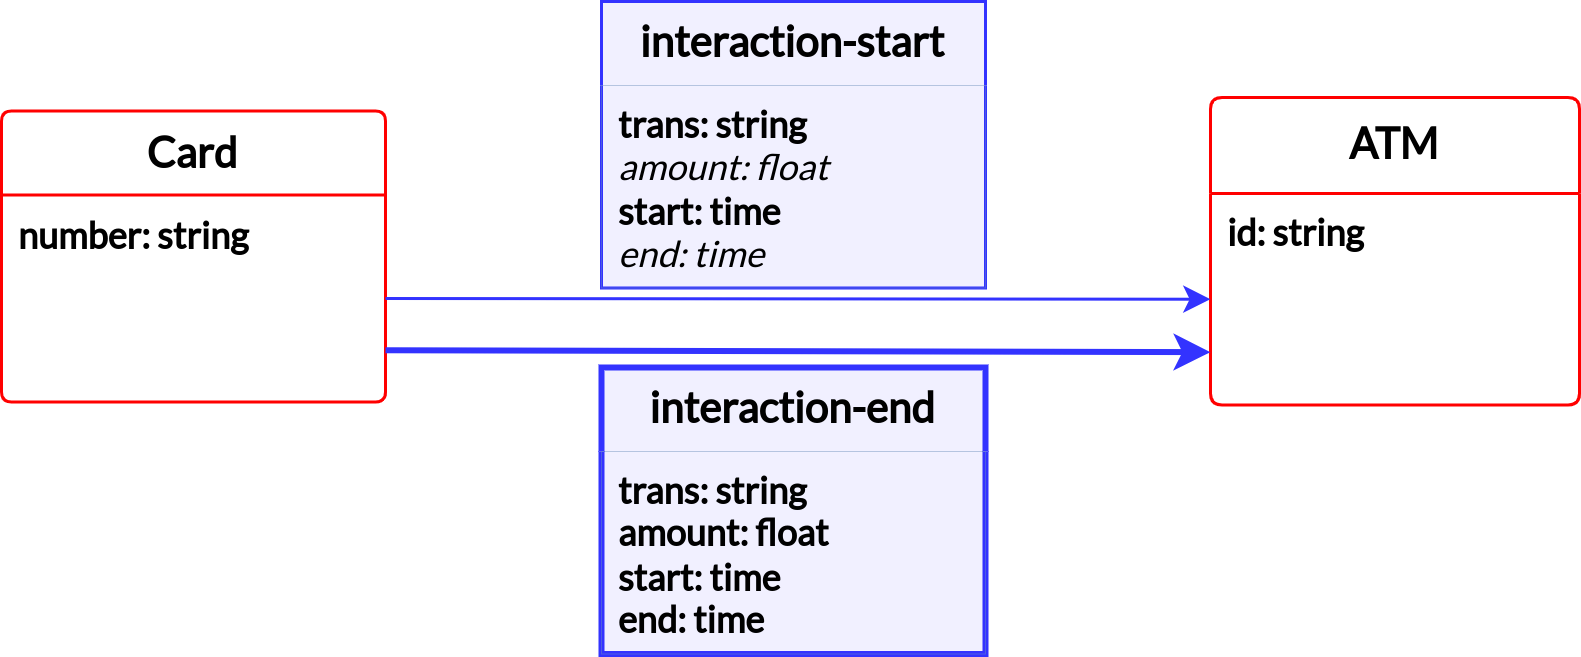
\includegraphics[width=\textwidth]{figures/2-edges-tx-end.png}}
    \caption{\only<1>{Opening edge}\only<2>{Closing edge}}
\end{figure}

\end{frame}

\end{comment}

\begin{frame}{Proposal: Definition of Anomalous Patterns of Transactions}
\begin{figure}
    \hspace*{-0.6cm}
    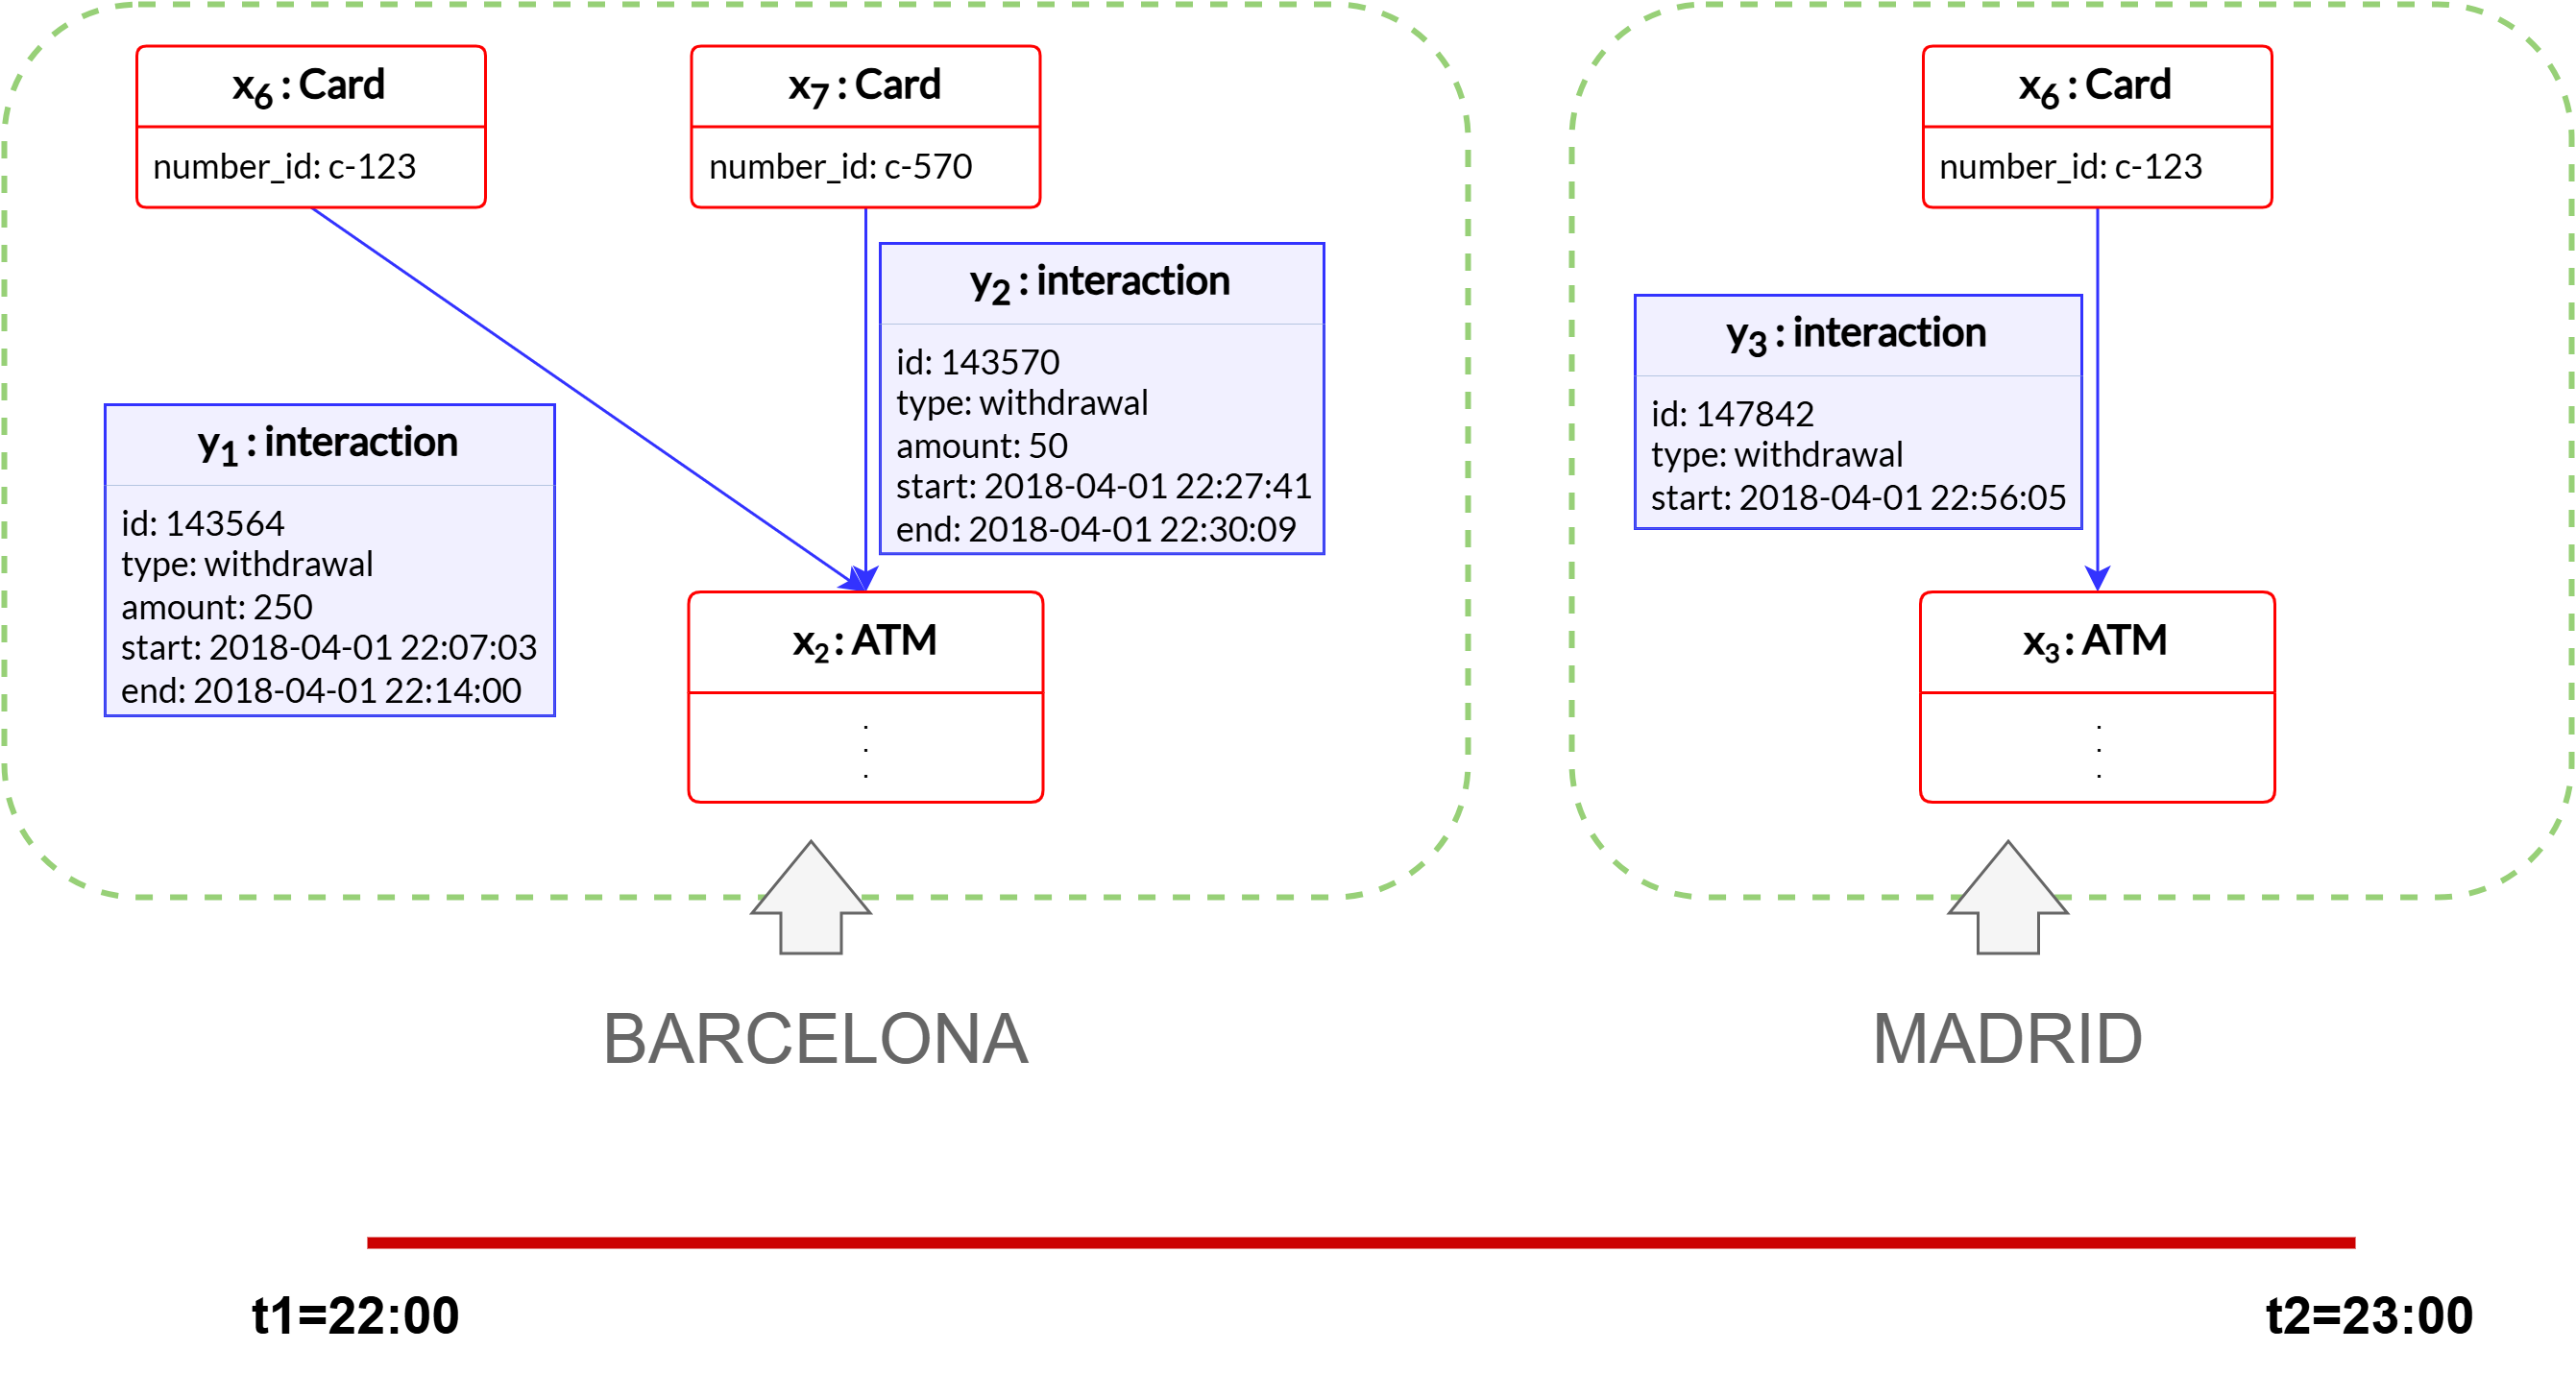
\includegraphics[width=1.10\textwidth]{images/2-QueryModel/FP1-Example.png}
    \caption*{Card cloning characterization - an example}
\end{figure}
\end{frame}

\begin{frame}{Proposal: Definition of Anomalous Patterns of Transactions}
\begin{itemize}
    \item Continuous queries are characterized as (constrained) \textbf{graph patterns}
\end{itemize}   
\begin{columns}
      % primera columna
      \begin{column}{0.3\textwidth}    
        \begin{figure}
            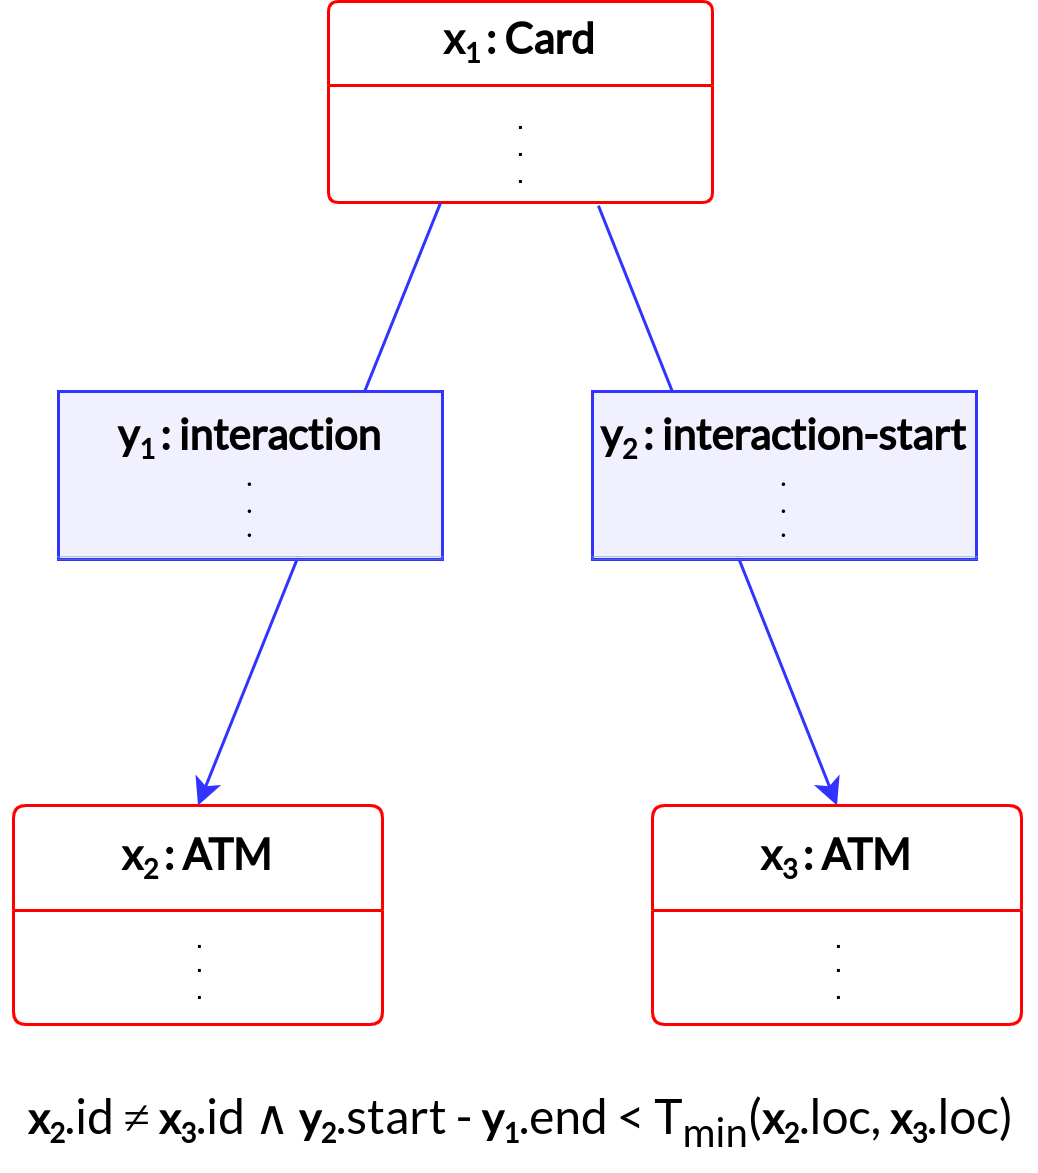
\includegraphics[scale=0.45]{images/2-QueryModel/graphPattern-1.png}
            \caption*{Card cloning}
        \end{figure}
      \end{column}
      \hfill
      % segunda columna
      \begin{column}{0.7\textwidth}   
        \vspace{1.5em}
        \begin{figure}
            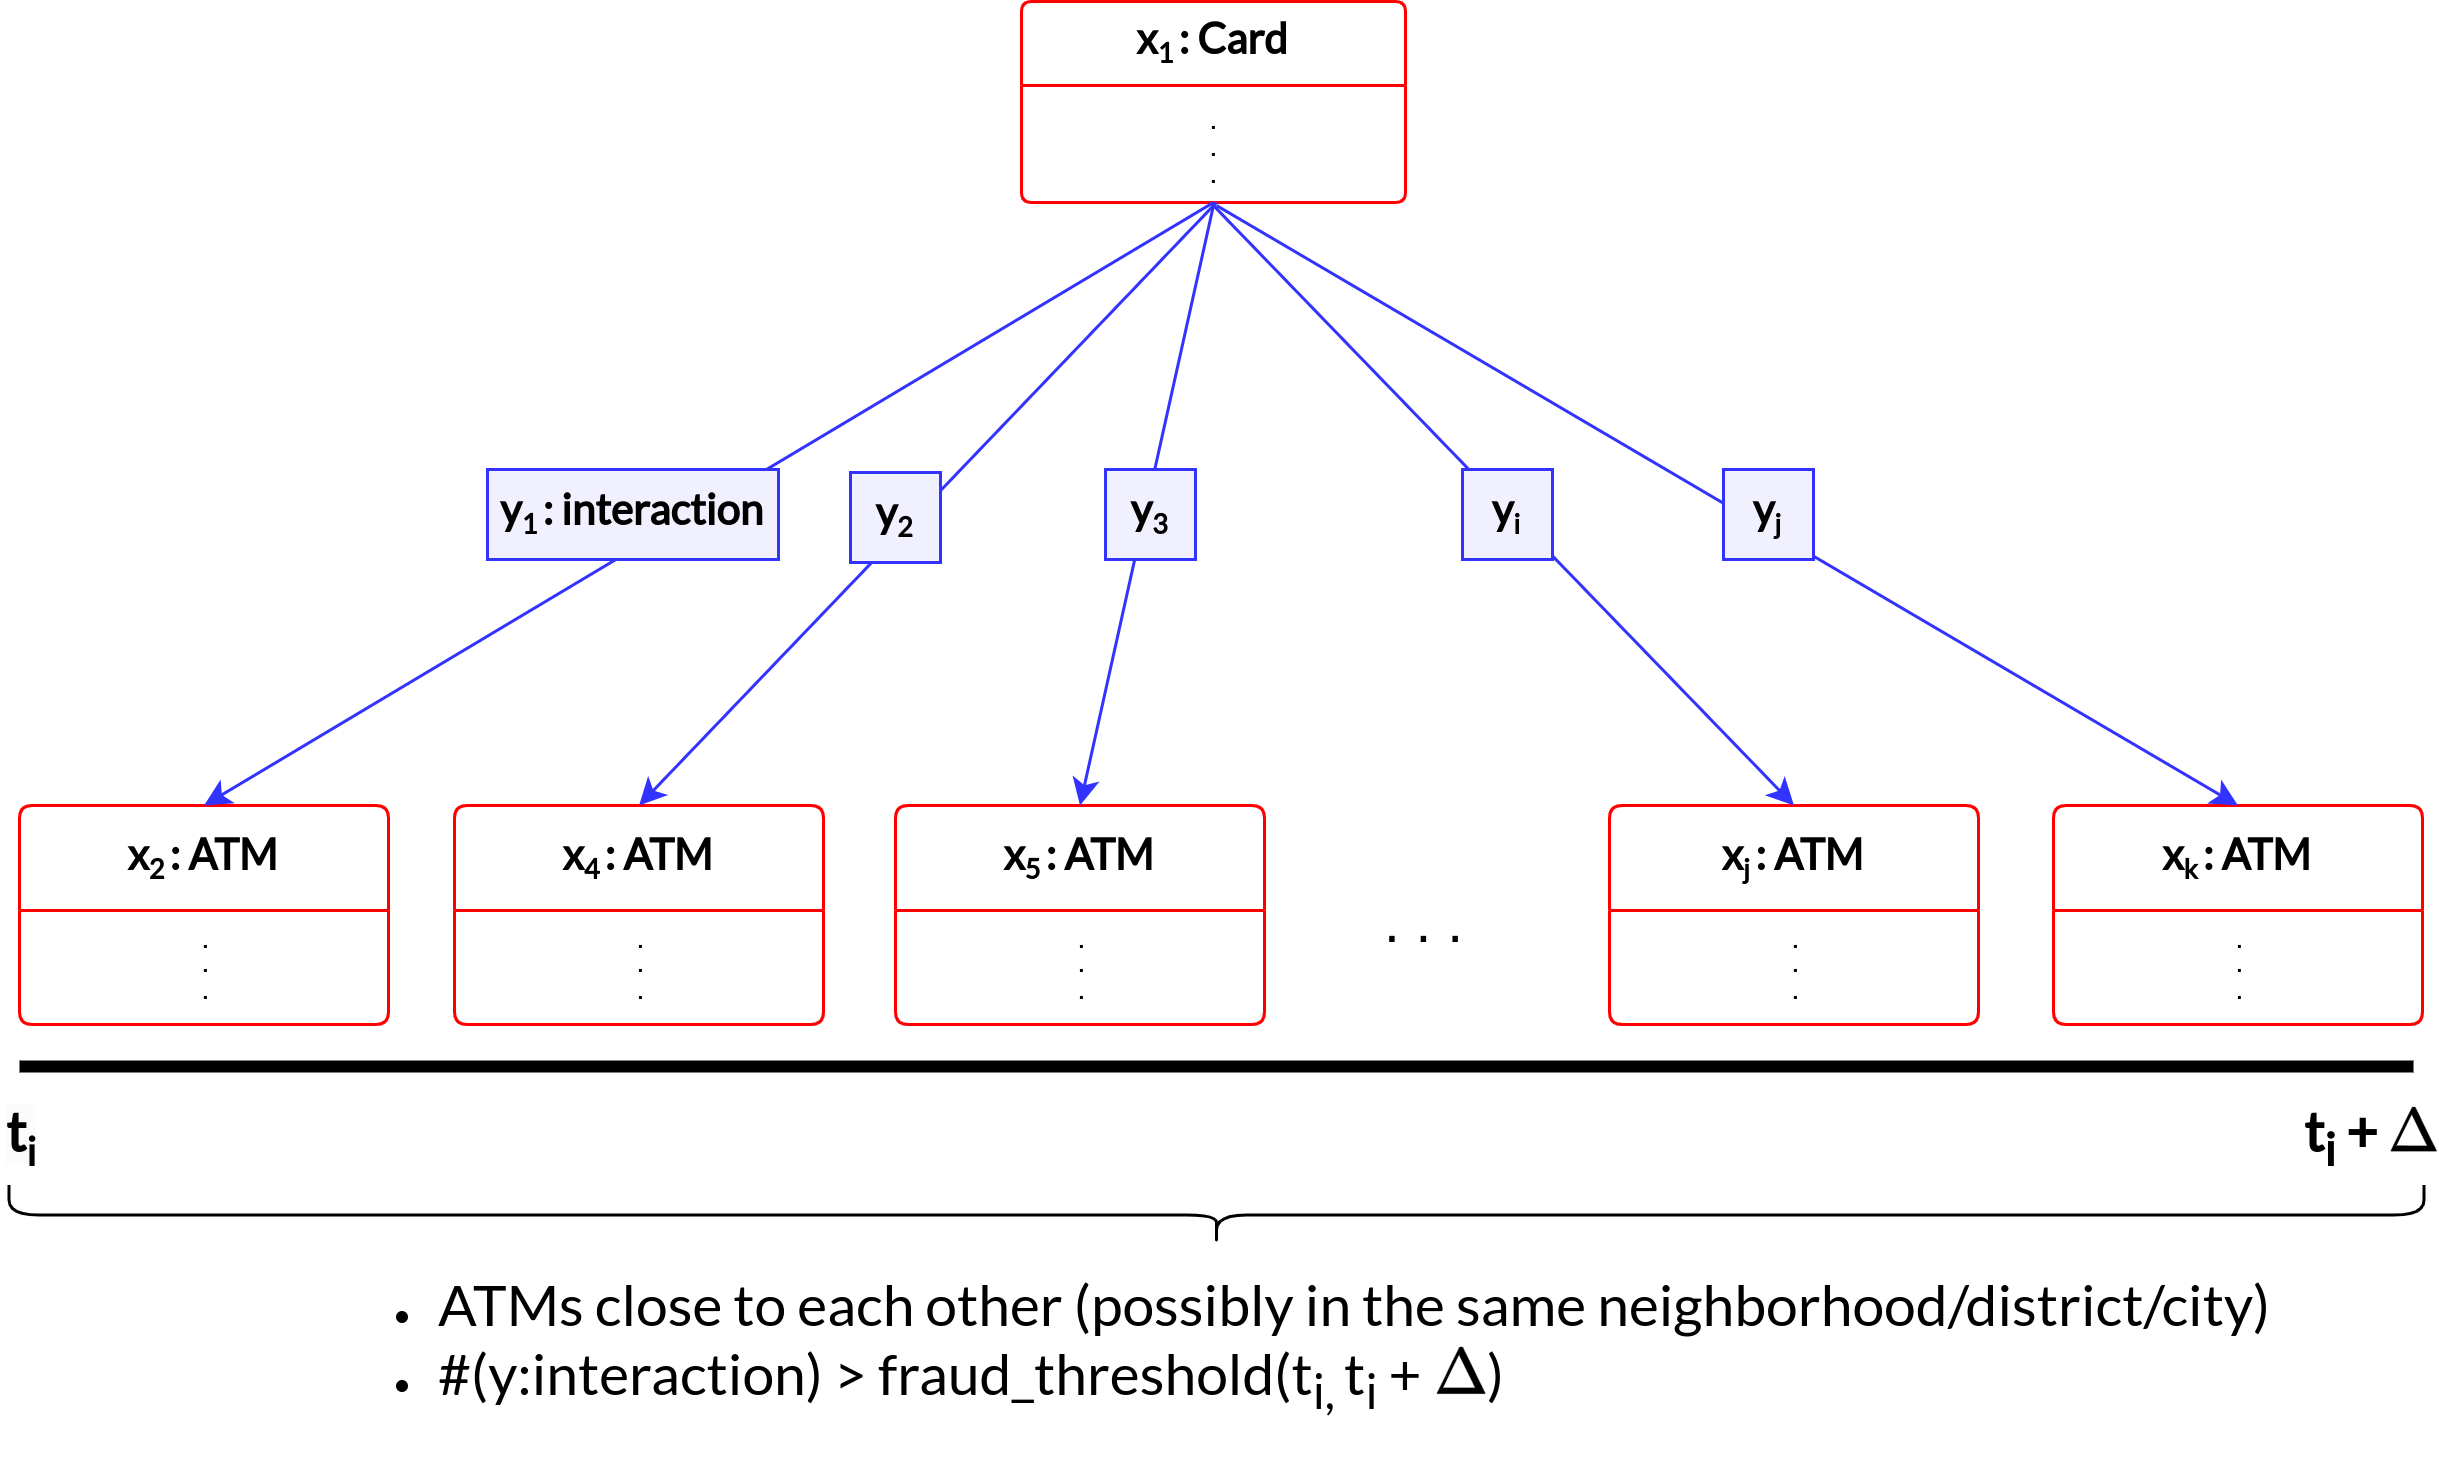
\includegraphics[scale=0.35]{images/2-QueryModel/graphPattern-2.png}
            \caption*{\emph{Lost-and-stolen} card}
        \end{figure}   
      \end{column}
\end{columns}
\end{frame}

\begin{frame}{Proposal: Query Model}
    \begin{itemize}
        \item \textbf{\emph{Continuous query model}}: Fixed queries evaluated over data streams.
        \item Progressive query evaluation process. Based on: \\
        \vspace{0.3em}
        \begin{itemize}
            \item \fbox{Graph pattern matching} in the \textcolor{blue}{volatile subgraph}. \\
            \item[\textcolor{black}{\ding{59}}\hspace*{-6em}] 
            \item \fbox{Satisfiability of constraints} over the properties: possibly querying the \textcolor{blue}{stable graph database} (\textit{retrieve some additional info}).
        \end{itemize}
    \end{itemize}
    \hspace*{1cm}
    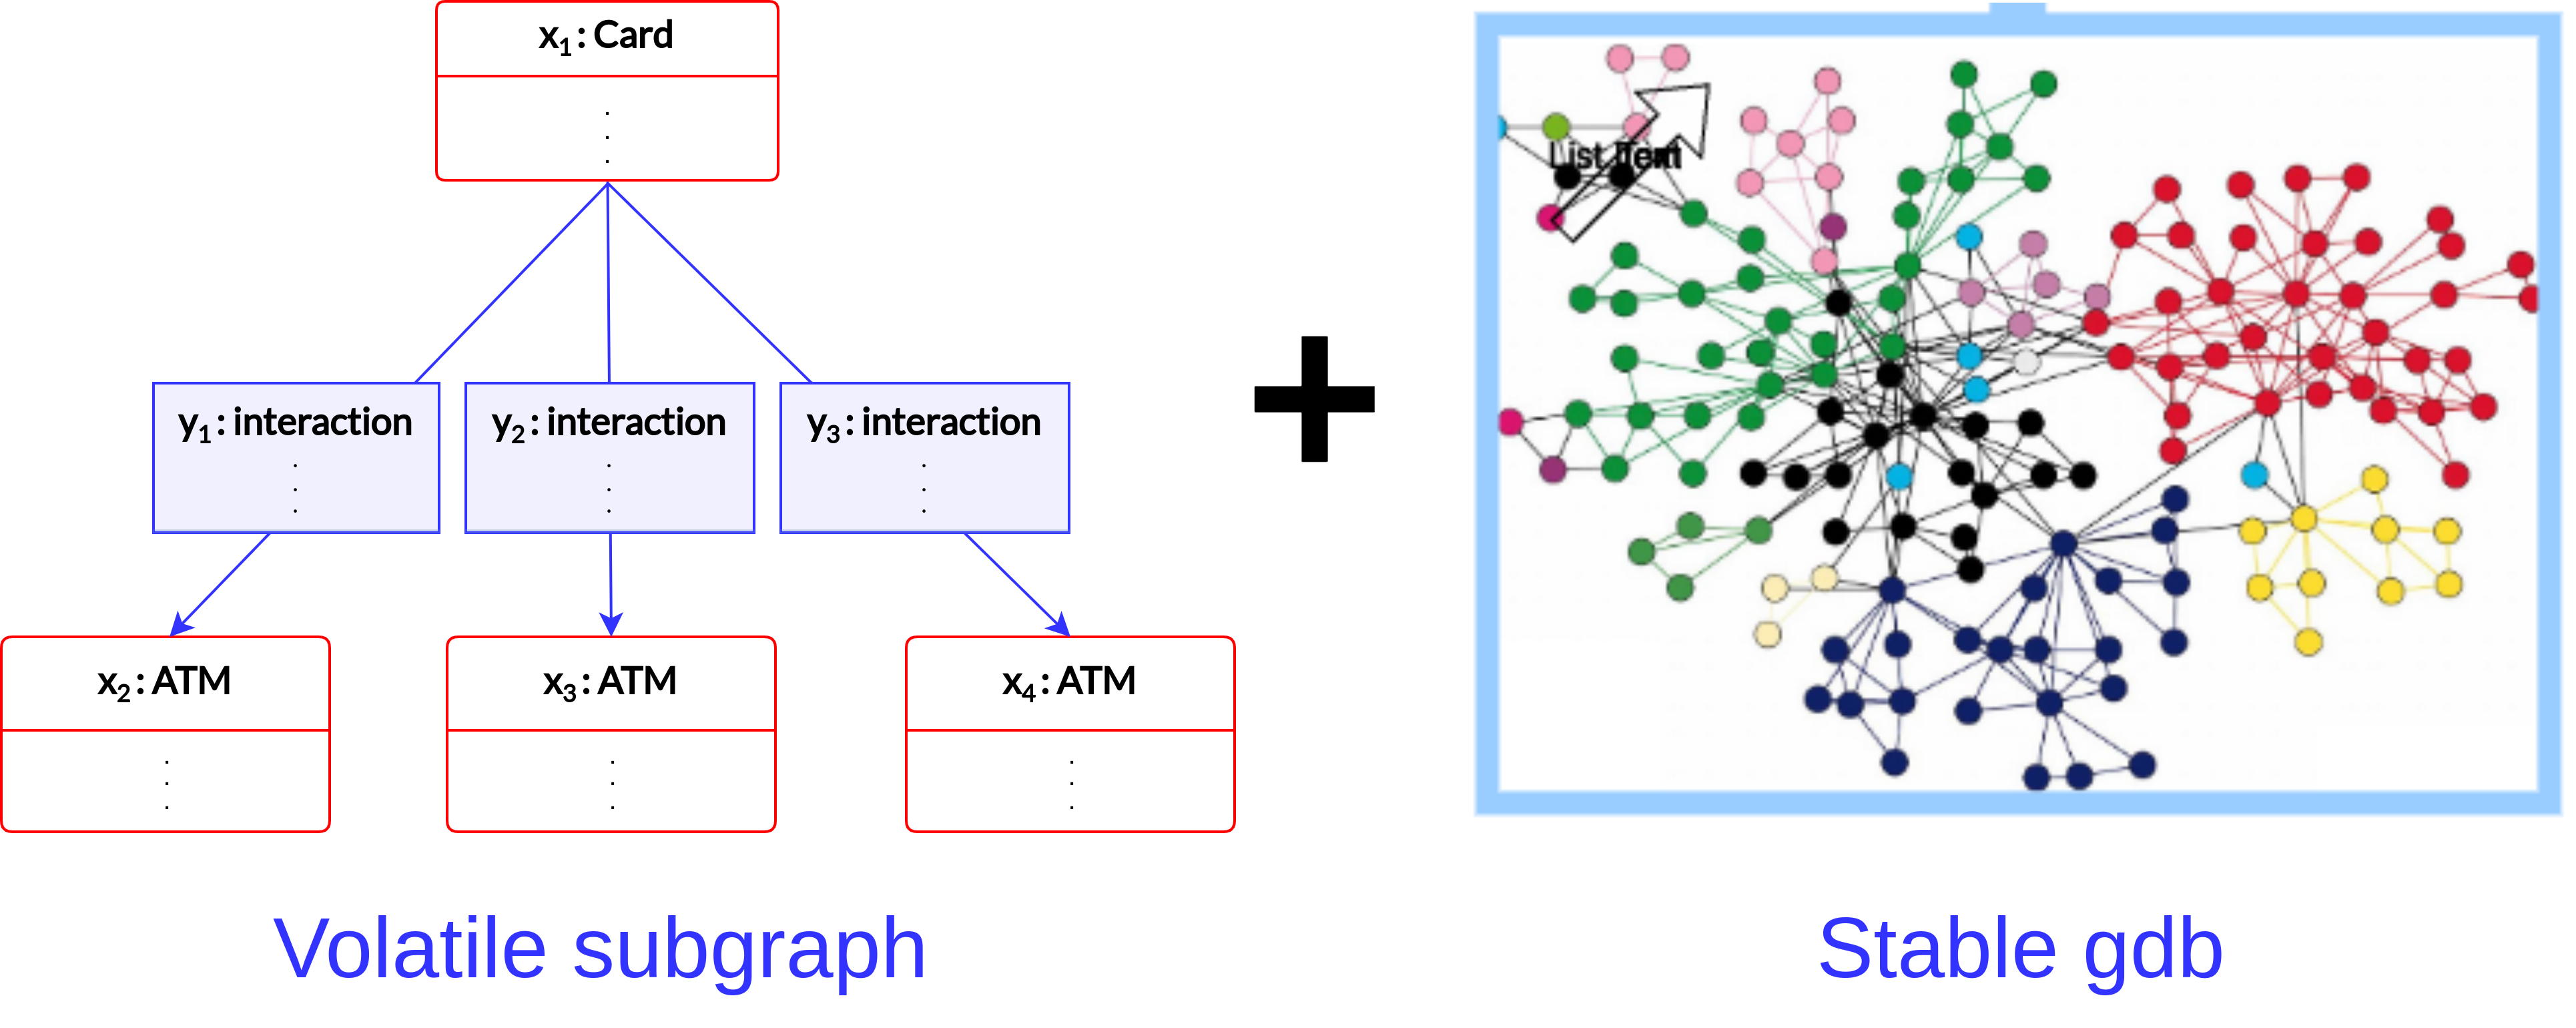
\includegraphics[scale=0.35]{figures/querymodel.png}
\end{frame}

\begin{frame}{Proposal: Continuous Query Engine - \DPATM}
\begin{itemize}
    \item Stream processing computational model. Dynamic Pipeline.
    \item Execution of tasks ({\small query evaluations}) concurrently/in-parallel.
\end{itemize}

\begin{figure}
    \hspace{-5.7cm}
    \centering
    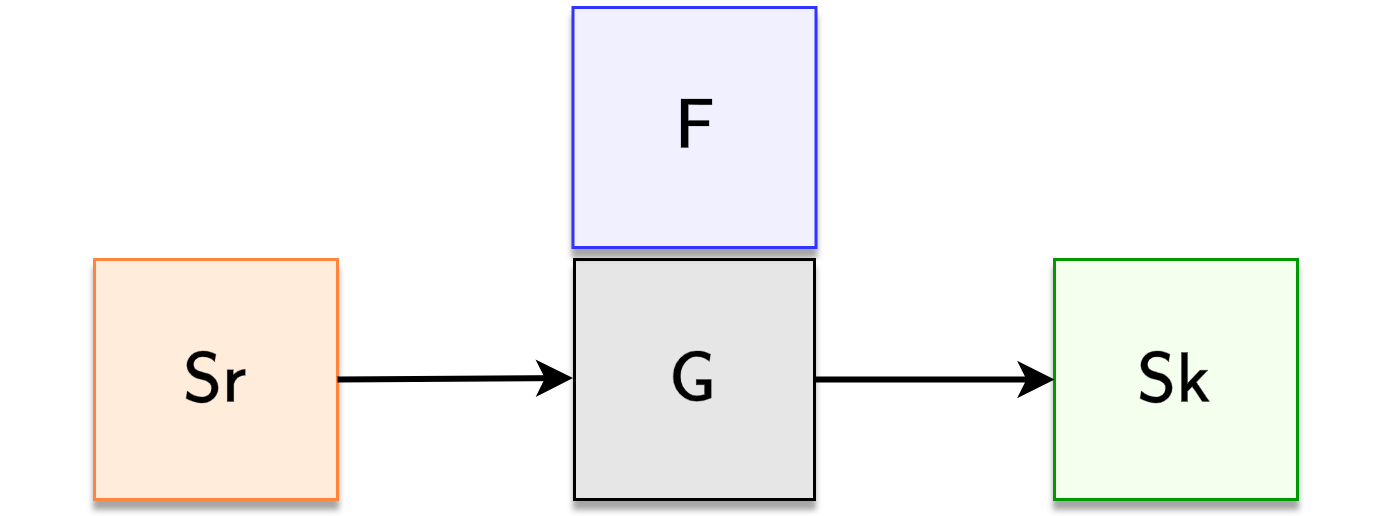
\includegraphics[width=0.55\linewidth]{images/3-Engine/DP-Stages-1.png}
\end{figure}
\begin{figure}
    \centering
    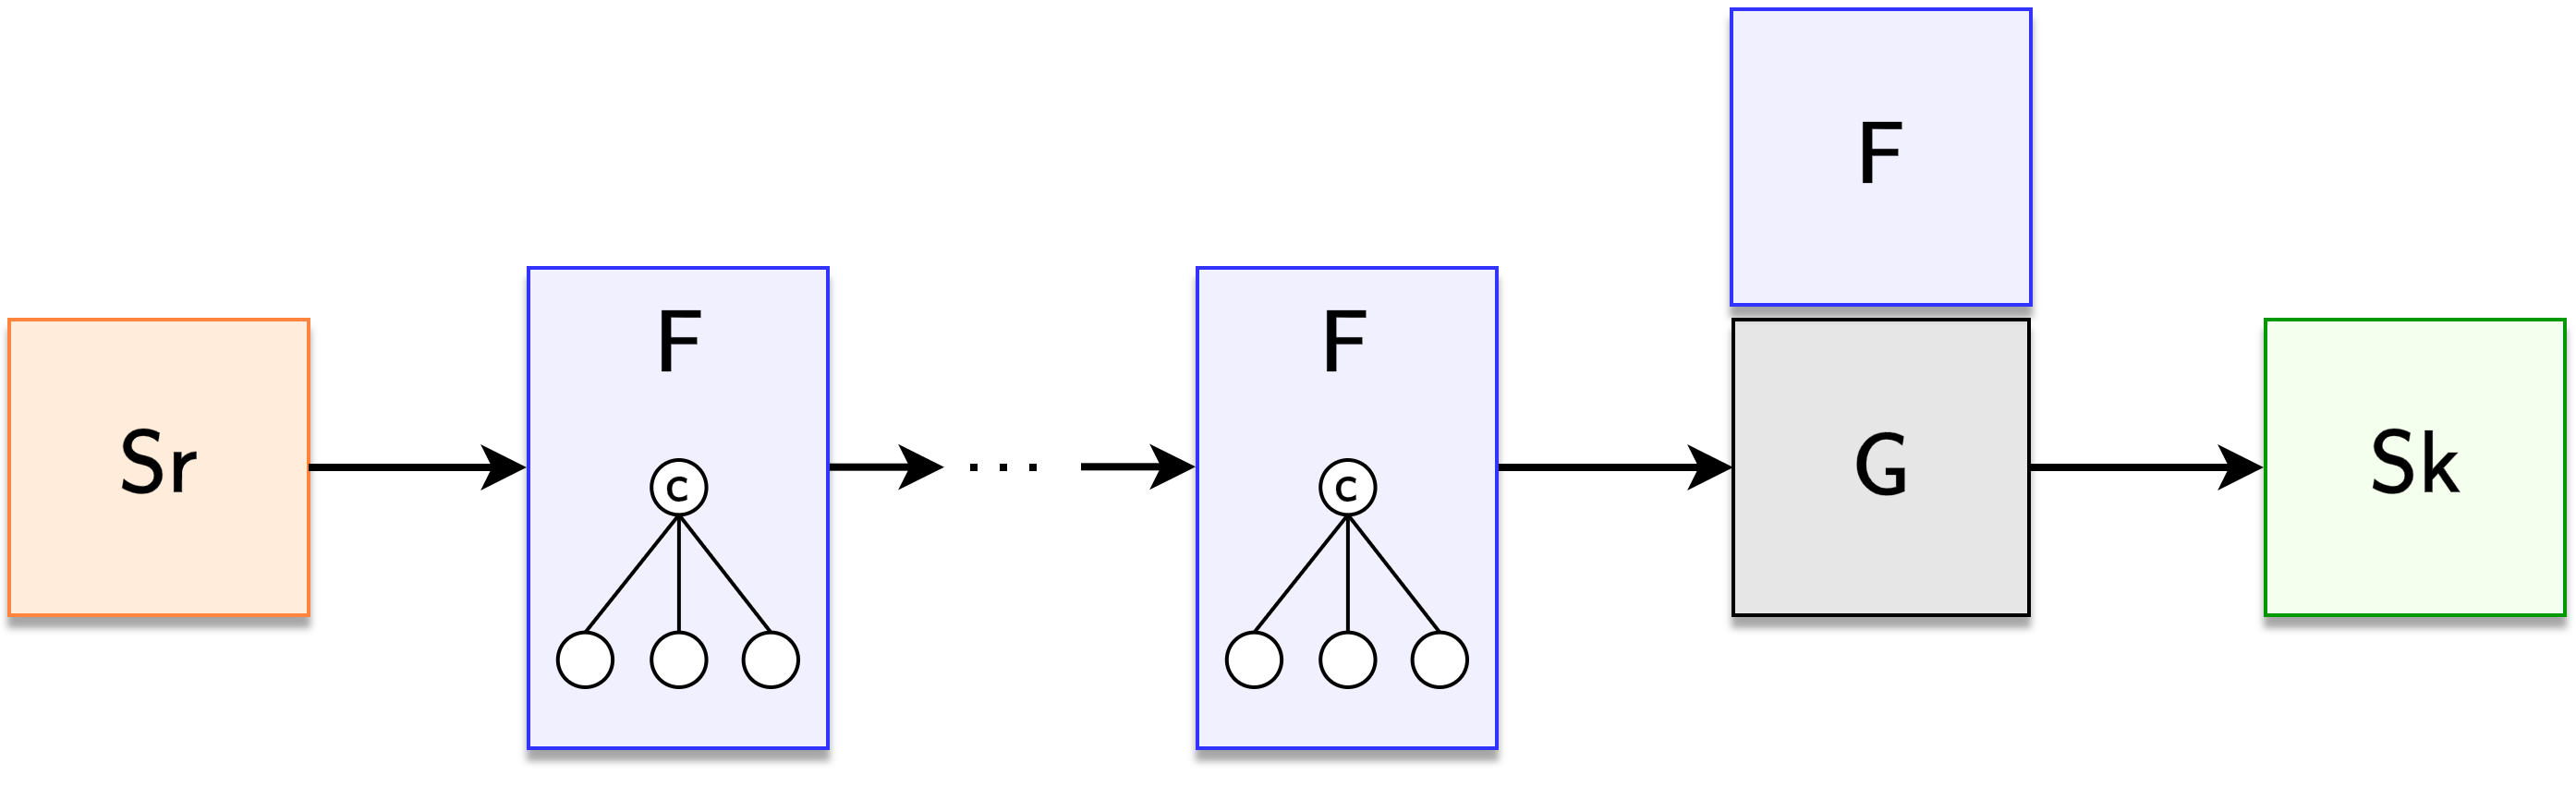
\includegraphics[width=1.0\linewidth]{figures/DP-FilterDetail-1.png}
\end{figure}


Based on \textbf{Dynamic Computational Approach} - {\footnotesize \cite{Pasarella2024}}. 


\end{frame}

\begin{comment}
 Royo-Sales \cite{DP-bitriangles2021}
%The problem of progressively identifying and enumerating bitriangles (i.e. a specific graph pattern) in bipartite evolving graphs using the DPA have been successfully solved by Royo-Sales \cite{DP-bitriangles2021}.
%\item Useful to address the problem of evaluating continuous queries over \emph{continuously evolving PGs} (Royo-Sales \cite{DP-bitriangles2021}).
\end{comment}


